\documentclass{beamer}
%\usepackage{beamerthemeshadow}
\beamersetuncovermixins{\opaqueness<1>{25}}{\opaqueness<2->{15}}
\setbeamertemplate{navigation symbols}{}
\usetheme{}
%\usecolortheme{seahorse}
\usepackage{graphicx}
\usepackage{fancyhdr}
\usepackage{ngerman}
\usepackage[T1]{fontenc}
\usepackage[latin1]{inputenc}
\usepackage{amsmath}
\usepackage{tabularx}
\usepackage{booktabs}
\usepackage{framed}

%\bibliographystyle{apalike}
%\usepackage{natbib}
\renewcommand{\figurename}{Abb.}
\setbeamercovered{transparent}





\title{Display multiple comparisons}
\subtitle{Journal Club}
\institute[Institute of Biostatistics]{Institute of Biostatistics\\ \url{andreaskitsche@gmail.com}}
\author{A. Kitsche}
\date{\today} 

\begin{document}


\frame{\titlepage}

%\frame{\tableofcontents}



\section{Types of Displays}
\begin{frame}
\frametitle{Types of Displays}
\begin{itemize}
\item Table with n rows, one for each comparison (summary statistic or CI)
\item Tiebreaker plot of the confidence intervals (\cite{Bretz.2010})
\item Compact letter display (\cite{Piepho.2004})
\item Mean-mean multiple comparison plot (\cite{Heiberger.2006, Heiberger.2010})
\end{itemize}
\end{frame}

\begin{frame}
\frametitle{Data set}
\begin{figure}
	\centering
		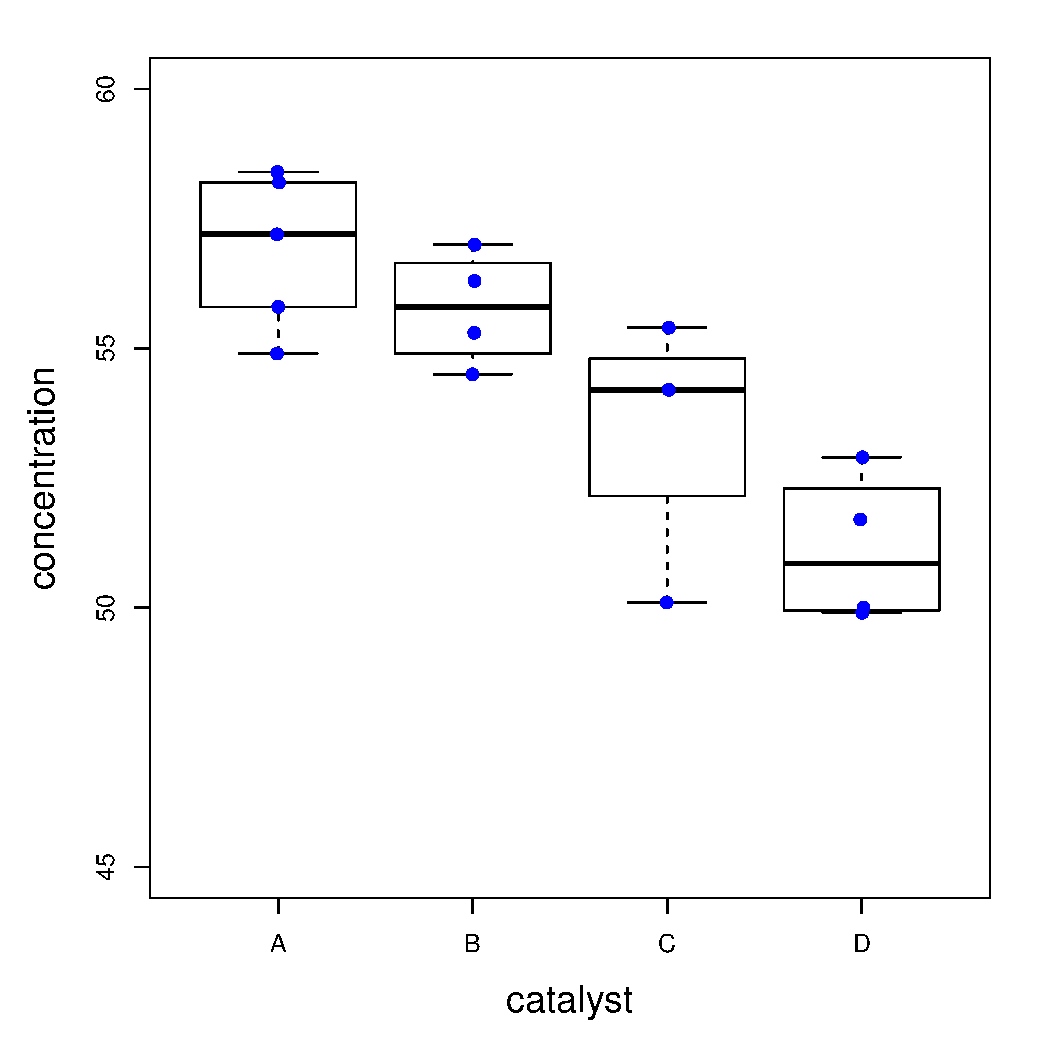
\includegraphics[width=0.80\textwidth]{Boxplot_catalyst.pdf}
	\label{fig:Boxplot_catalyst}
\end{figure}

\end{frame}



\begin{frame}
\frametitle{Table with n rows, one for each comparison (summary statistics)}
\begin{table}
\begin{tabular}{lrrrl}
           &Estimate& Std. Error& t value& Pr(>|t|)\\   
B - A == 0&   -1.125&      1.138&  -0.988&  0.75812\\   
C - A == 0&   -3.667&      1.239&  -2.958&  0.05060 .\\ 
D - A == 0&   -5.775&      1.138&  -5.073&  0.00142 **\\
C - B == 0&   -2.542&      1.296&  -1.961&  0.25474 \\  
D - B == 0&   -4.650&      1.200&  -3.875&  0.01021 *\\ 
D - C == 0&   -2.108&      1.296&  -1.627&  0.40012 
\end{tabular}
\end{table} 
\end{frame}

\begin{frame}
\frametitle{Table with n rows, one for each comparison (Confidence intervals)}
\begin{table}
\begin{tabular}{lrrr}
         & Estimate& lwr&      upr\\     
B - A == 0& -1.12500& -4.50306&  2.25306\\
C - A == 0& -3.66667& -7.34423&  0.01090\\
D - A == 0& -5.77500& -9.15306& -2.39694\\
C - B == 0& -2.54167& -6.38776&  1.30442\\
D - B == 0& -4.65000& -8.21079& -1.08921\\
D - C == 0& -2.10833& -5.95442&  1.73776
\end{tabular}
\end{table} 
\end{frame}

\begin{frame}
\frametitle{Tiebreaker plot of the confidence intervals}
\begin{figure}
	\centering
		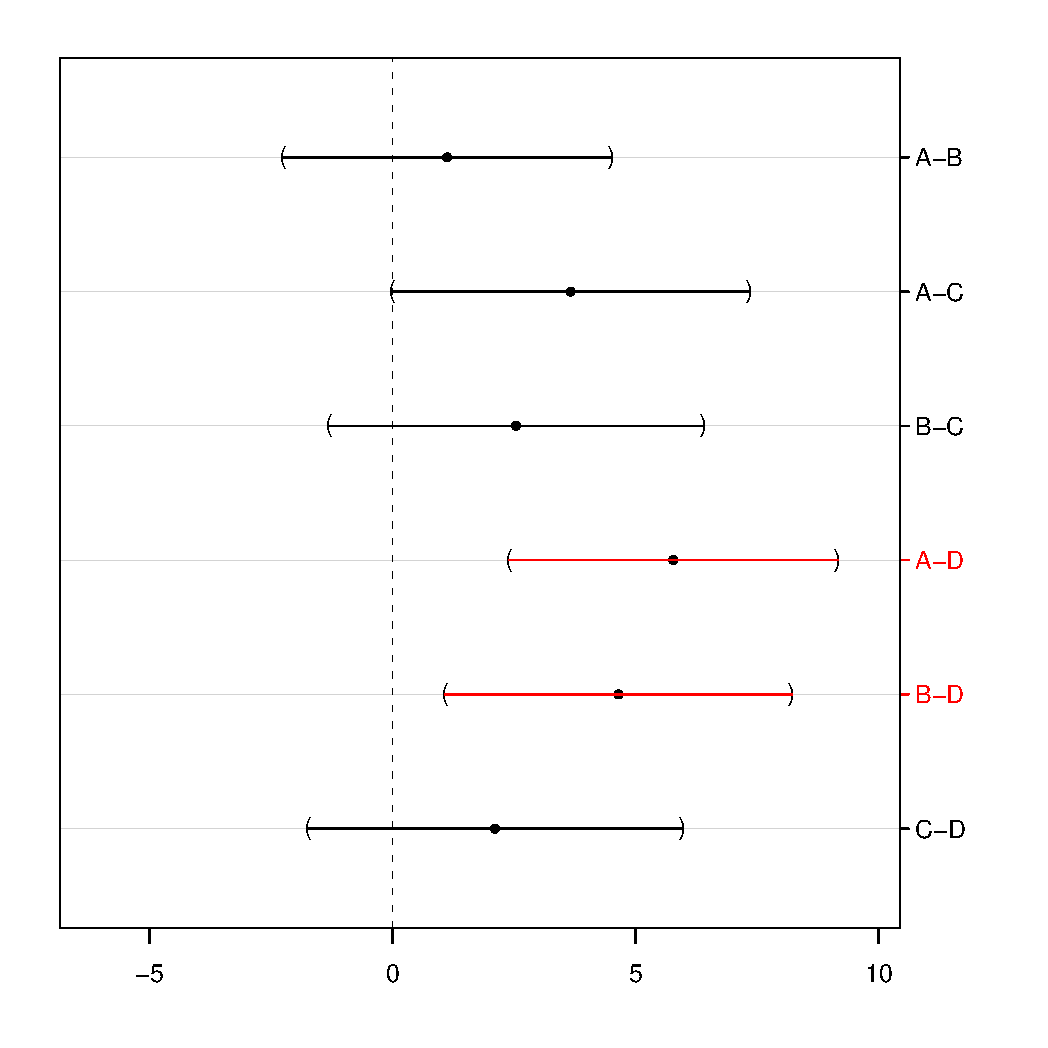
\includegraphics[width=0.80\textwidth]{CI_catalyst.pdf}
	\label{fig:CI_catalyst}
\end{figure}

\end{frame}

\begin{frame}
\frametitle{Compact letter display - 1}
\begin{figure}
	\centering
		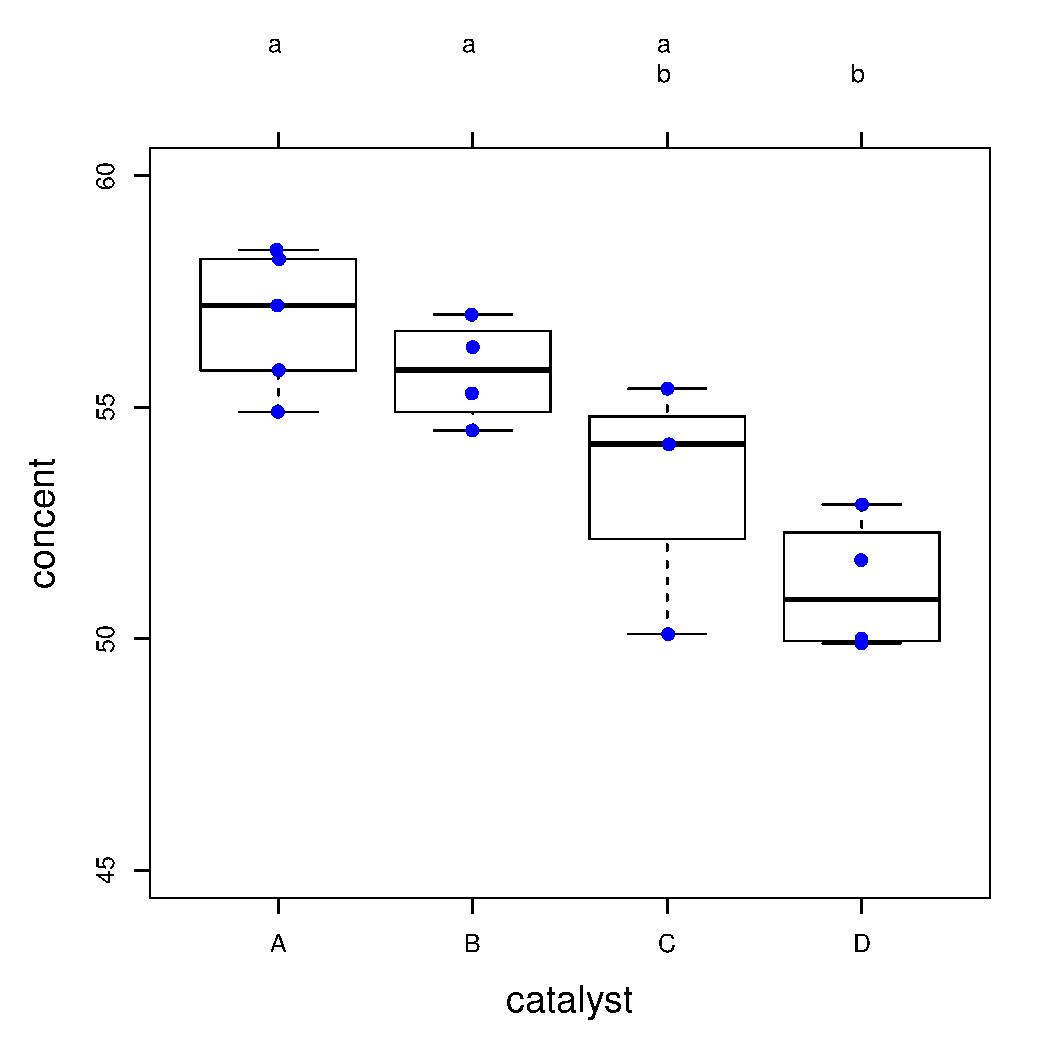
\includegraphics[width=0.80\textwidth]{cld_catalyst.pdf}
	\label{fig:cld_catalyst}
\end{figure}
\end{frame}

\begin{frame}
\frametitle{Compact letter display - 2}
\begin{figure}
	\centering
		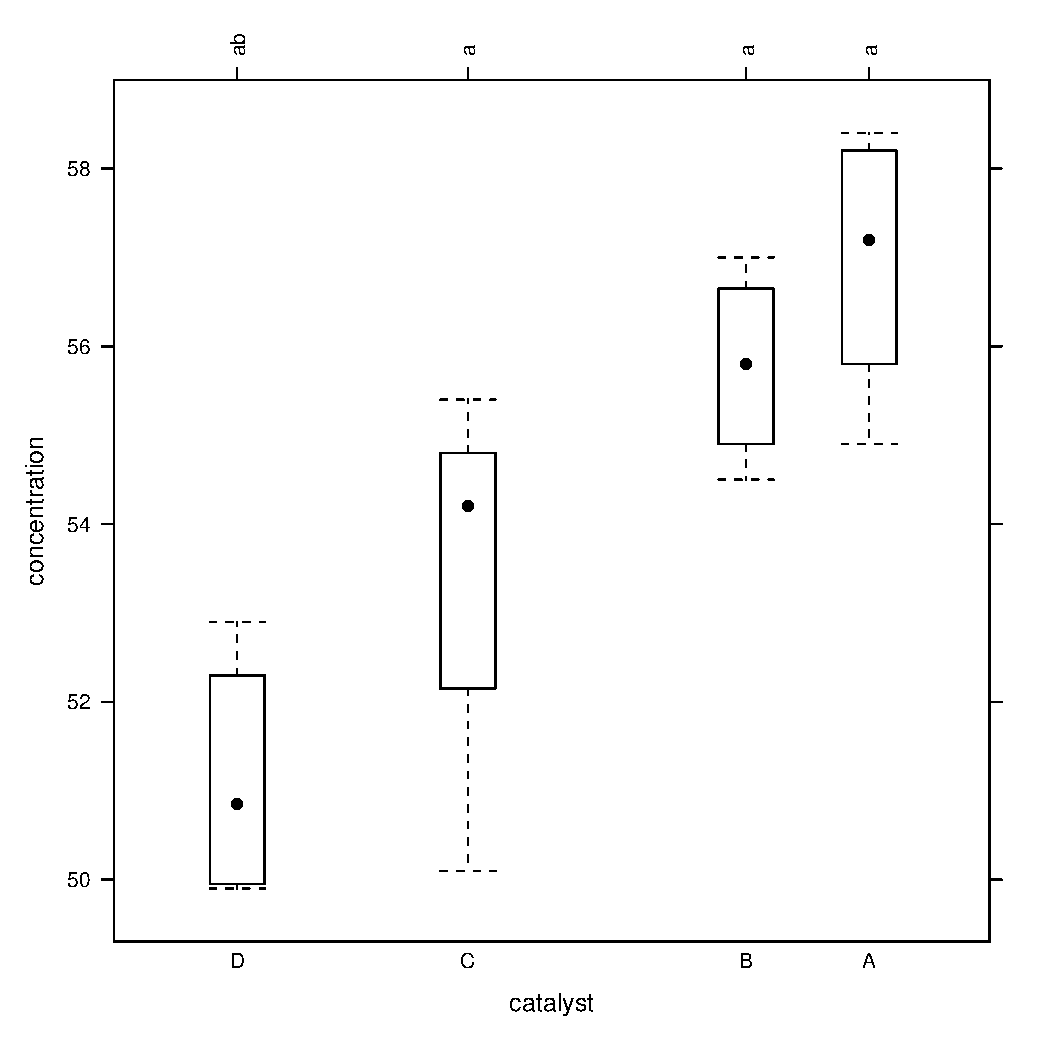
\includegraphics[width=0.80\textwidth]{Boxplot_catalystBretz.pdf}
	\label{fig:cld2_catalyst}
\end{figure}
\end{frame}

\begin{frame}
Existing procedures for graphically presenting the results of such procedures suffer from
an inability to show all of the relevant information in the same plot:
\begin{itemize}
\item The sample means themselves, with correct relative distances 
\item The point and interval estimates of the pairwise differences
\item The point and interval estimates for arbitrary contrasts of the level means
\item Declarations of significance
\item Confidence interval widths that are correct for unequal sample sizes
\end{itemize}
\end{frame}

\begin{frame}
\frametitle{Construction of mean-mean multiple comparison plots - 1}
\begin{figure}
	\centering
		\includegraphics[width=1.00\textwidth]{mmc1-a.jpg}
	\label{fig:MMC1}
\end{figure}
\end{frame}

\begin{frame}
\frametitle{Construction of mean-mean multiple comparison plots - 2}
\begin{figure}
	\centering
		\includegraphics[width=1.00\textwidth]{mmc1-b0.jpg}
	\label{fig:MMC2}
\end{figure}
\end{frame}

\begin{frame}
\frametitle{Construction of mean-mean multiple comparison plots - 3}
\begin{figure}
	\centering
		\includegraphics[width=1.00\textwidth]{mmc1-b.jpg}
	\label{fig:MMC3}
\end{figure}
\end{frame}


\begin{frame}
\frametitle{Applications of MMC plots}
\begin{figure}
	\centering
		\includegraphics[width=1.00\textwidth]{mmc2.jpg}
	\label{fig:MMC4}
\end{figure}
\end{frame}


\begin{frame}
\frametitle{Applications of MMC plots}
\begin{figure}
	\centering
		\includegraphics[width=0.80\textwidth]{MMC_Tukeycatalyst}
	\label{fig:MMC5}
\end{figure}
\end{frame}

\begin{frame}
\frametitle{Applications of MMC plots}
\begin{figure}
	\centering
		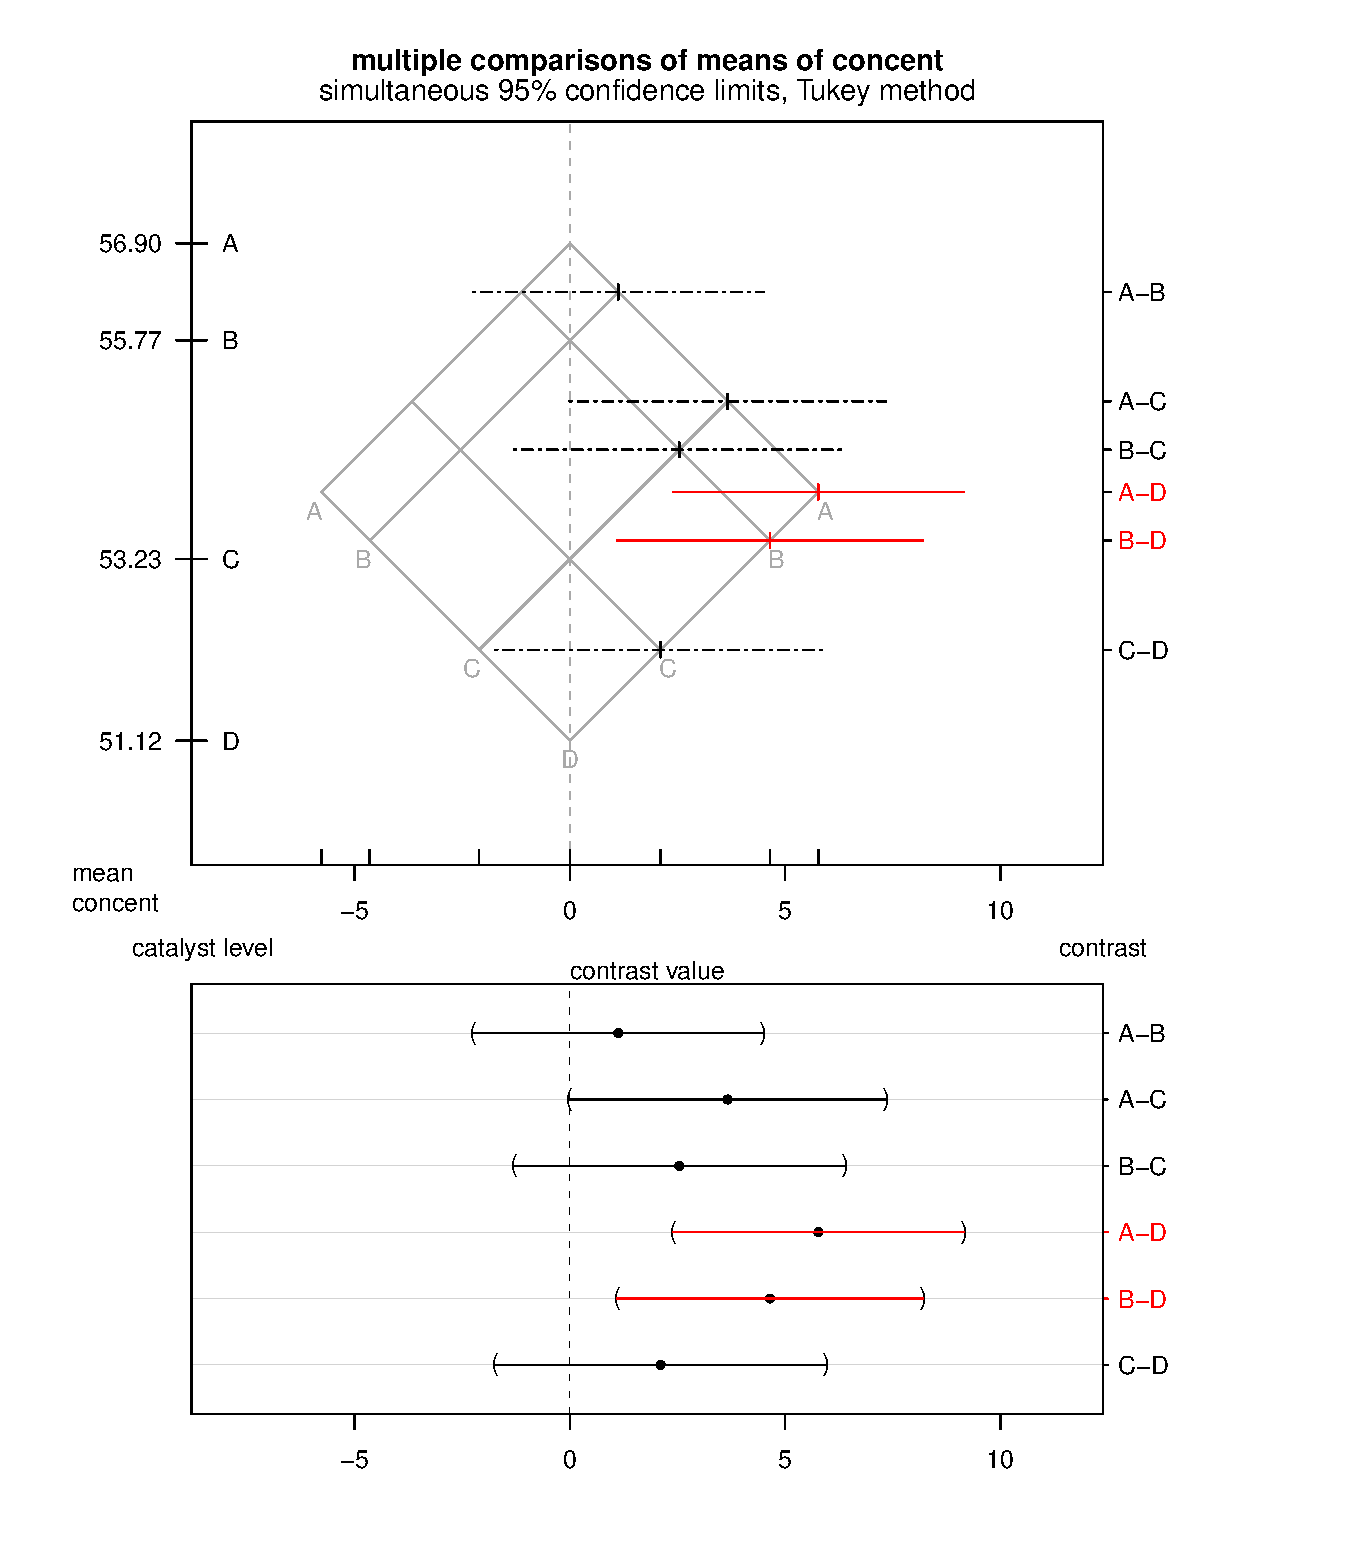
\includegraphics[width=0.60\textwidth]{CI_catalyst_comparison}
	\label{fig:MMC6}
\end{figure}
\end{frame}



\begin{frame}
\frametitle{\texttt{R} implementation}
function: \texttt{glht.mmc} with arguments:
\renewcommand{\labelitemi}{>}
\begin{itemize}
	\item \texttt{model} -	"`aov"' object in "`lm"' method
	\item \texttt{ylabel} -	name of the response variable
	\item \texttt{lmat} -	contrast matrix
\end{itemize}

\end{frame}



\footnotesize
\section{Literatur}
\setcounter{page}{1}
\pagenumbering{roman}
\bibliographystyle{plainnat}
\bibliography{MMC_Plot}


\end{document}

